\documentclass[]{article}

\usepackage{acro}
\usepackage{listings}
\usepackage{cleveref}
\usepackage{xcolor}
\usepackage{graphicx}

\definecolor{superlightgray}{rgb}{0.9, 0.9, 0.9} 

\lstset{
	numbers=left,
	stepnumber=1, 
	backgroundcolor=\color{superlightgray},
	basicstyle=\footnotesize,
	breaklines=false,
	rulecolor=\color{black},
	commentstyle=\color{blue},
	keywordstyle=\color{red},
	numberstyle=\scriptsize\color{black},
	stringstyle=\color{purple},
	columns=fullflexible
}

\DeclareAcronym{fov}{
	short = FOV,
	long = {Field of View}
}

\graphicspath{{../images_report/}}

\title{Ray-tracing based renderer from scratch in Python}
\author{Jörn Lasse Vaupel}
\date{\today}

\begin{document}
	
	\maketitle
	\newpage
	\tableofcontents
	
	\begin{abstract}
		
	\end{abstract}

	\newpage
	
	\section{Introduction}
	\label{sec:intro}
	This report summarizes the process of implementing a ray-tracing based renderer from scratch following the introduction from Peter Shirley’s Ray Tracing in One Weekend  \cite{Shirley2020RTW1} and its continuation Ray Tracing: The Next Week \cite{Shirley2020RTW2}. While Shirley used C++ as a high performance and efficiency programming language, the following implementation is written in Python.  Even if the rendering times may be longer, Python’s readability and easiness helps focusing on the basic concepts of ray-tracing based rendering. In addition, efficiency might be higher if the advantages of Python libraries like \emph{NumPy} would be used more strictly, but the focus of the implementation is on understanding, not on efficiency. All in all, some functions are just easier in Python than in C++.
	\\
	In the working process many different test images were rendered. In order to meet all the requirements for the final result and generate a uniformly growing scene, the implementation was completed before rendering the final images taking into account a backwards compatibility. Therefore, all final images can be generated by using the same structure: a scene containing one or several cameras and some spheres. Only the single-colored image is generated differently due to the gamma correction. This shows some design decisions in the implementation like a horizontal \ac{fov} or gamma correction, can lead to slightly different results than those, that were possible in previous stages of implementation. This is no big deal but should be mentioned.
	
	\section{First rendering loop}
	Just with the beginning the first example of understanding against efficiency occurs. In order to speed up rendering and to limit the amount of file accesses, the rendered image is saved in an image array maintained by an \emph{Image} class before saved in a .ppm file. The rendering loop requires a double for loop. To avoid generating the file from scratch within another double for loop, it’s possible to use Python libraries like \emph{Pillow} to directly write a .ppm file. But to enable a deeper understanding of the structure of the file format while utilizing the advantages of Python libraries, a custom approach based on \emph{NumPy} is used (the double for loop approach is also shown but not used).
	\\
	The code from \emph{scene1.py} in \cref{lst:first_render_loop} shows the basic use of the \emph{Image} class and the render loop which generates the image in \cref{fig:image1}. The render loop will be later handled by the \emph{Camera} class.
	
	\begin{lstlisting}[caption={Example for a basic render loop}, language=Python, label=lst:first_render_loop]
image = Image(1920, 1080)
for y in range(image.height)[::-1]:
	for x in range(image.width):
		image.image_list[y, x] = Vector(128, 64, 255).to_int_array()

image.save_image("../images/image1.ppm")
	\end{lstlisting}

	\begin{figure}[h]
		\centering
		
\includegraphics[width=0.75\linewidth]{image1}
		\caption{Singe-colored image generated by first render loop}
		\label{fig:image1}
	\end{figure}

	\section{Camera}
	The implementation of the camera in the \emph{Camera} class largely follows the tutorial in \cite{Shirley2020RTW1}. In general, it’s necessary to define a large set of algebraic methods within the \emph{Vector} and \emph{Ray} class. Referring the \emph{Vector} class, it’s important to mention that the default operators (e.g. \textbf{+} and \textbf{-}) are overloaded and especially the meaning of \textbf{*} operator depends on the second operand. If it’s a float the operation defines a scalar multiplication, if it’s a vector the result is the dot product of both vectors.
	\\
	A small addition to the concept in \cite{Shirley2020RTW1} used in this implementation is the idea that every object within a 3D scene has a position (and a rotation) and can therefore be described as an object of a common class: the \emph{Transform} class. This does not grant any advantages now but makes the implementation of new 3D objects like spheres (or maybe a collection of planes in future) easier.
	\\
	The resulting image is shown in \cref{fig:image2}. Because of the lag of backwards compatibility described in \cref{sec:intro} or - to be more precisely - due to personal favor, the \ac{fov} is slightly different in all rendered images. The default horizontal \ac{fov} is set to $130^{\circ}$ (representing human horizontal \ac{fov}), while the \ac{fov} $\phi$ in \cite{Shirley2020RTW1} results from focal length $fl=1$, viewport height $vp_h=2$ and aspect ratio $ar=\label{key}16/9$ as shown in \cref{equ:fov}.
	\begin{equation}
		\label{equ:fov}
		\phi = 2\cdot arctan\left(\frac{vp_h\cdot ar}{2\cdot fl}\right) \approx 121,28^{\circ}
	\end{equation}
	
	\begin{figure}[h]
		\centering
		
\includegraphics[width=0.75\linewidth]{image2}
		\caption{Gradient image generated by camera (empty 3D scene)}
		\label{fig:image2}
	\end{figure}

	\section{Spheres}
	Just like the implementation of the camera the implementation of spheres within the \emph{Sphere} class was straight forward understanding the concepts from \cite{Shirley2020RTW1} and transfer them to Python. Key feature is the \emph{hit(ray, t\textunderscore min, t\textunderscore max)} function every 3D object which can interact with camera rays must have. Therefore the class \emph{RenderObject} is defined which inherits from \emph{Transform} class and provides an abstract function \emph{hit(ray, t\textunderscore min, t\textunderscore max)}. That function later has to be implemented by the sub classes of \emph{RenderObject} like \emph{Sphere}.
	\\
	In case of the \emph{Sphere} class the intersection of ray and sphere is calculated using an optimized equation based on the radius and position of the sphere. Because most of the times two intersections will be detected for each ray, only the closer point is used. The function also returns the normal in the intersection point and flips it if the ray was emitted from within the sphere. On this place the implementation varies from the approach in \cite{Shirley2020RTW1}. The ray is outside the sphere if the dot product of the ray’s direction and the normal in the intersection point is greater than or equal to 0 (if both are orthogonal it’s still outside), while there is only $<$ used in \cite{Shirley2020RTW1}. For numerical approaches this makes no big difference, because this case rarely occurs but for correctness and understanding this was changed (logical difference between Listing 17 and Listing 18 in \cite{Shirley2020RTW1}).
	\\
	The \emph{hit(ray, t\textunderscore min, t\textunderscore max)} also allows to limit the render distance by the \emph{t} parameters (close and far range) and returns color (or later material) of the sphere.
	\\
	Adding five spheres of different radius and color to a 3D scene of \emph{Scene} class (described in \cref{sec:scene}) results in a rendered image like in \cref{fig:image3}.
	
	\begin{figure}[h]
		\centering
		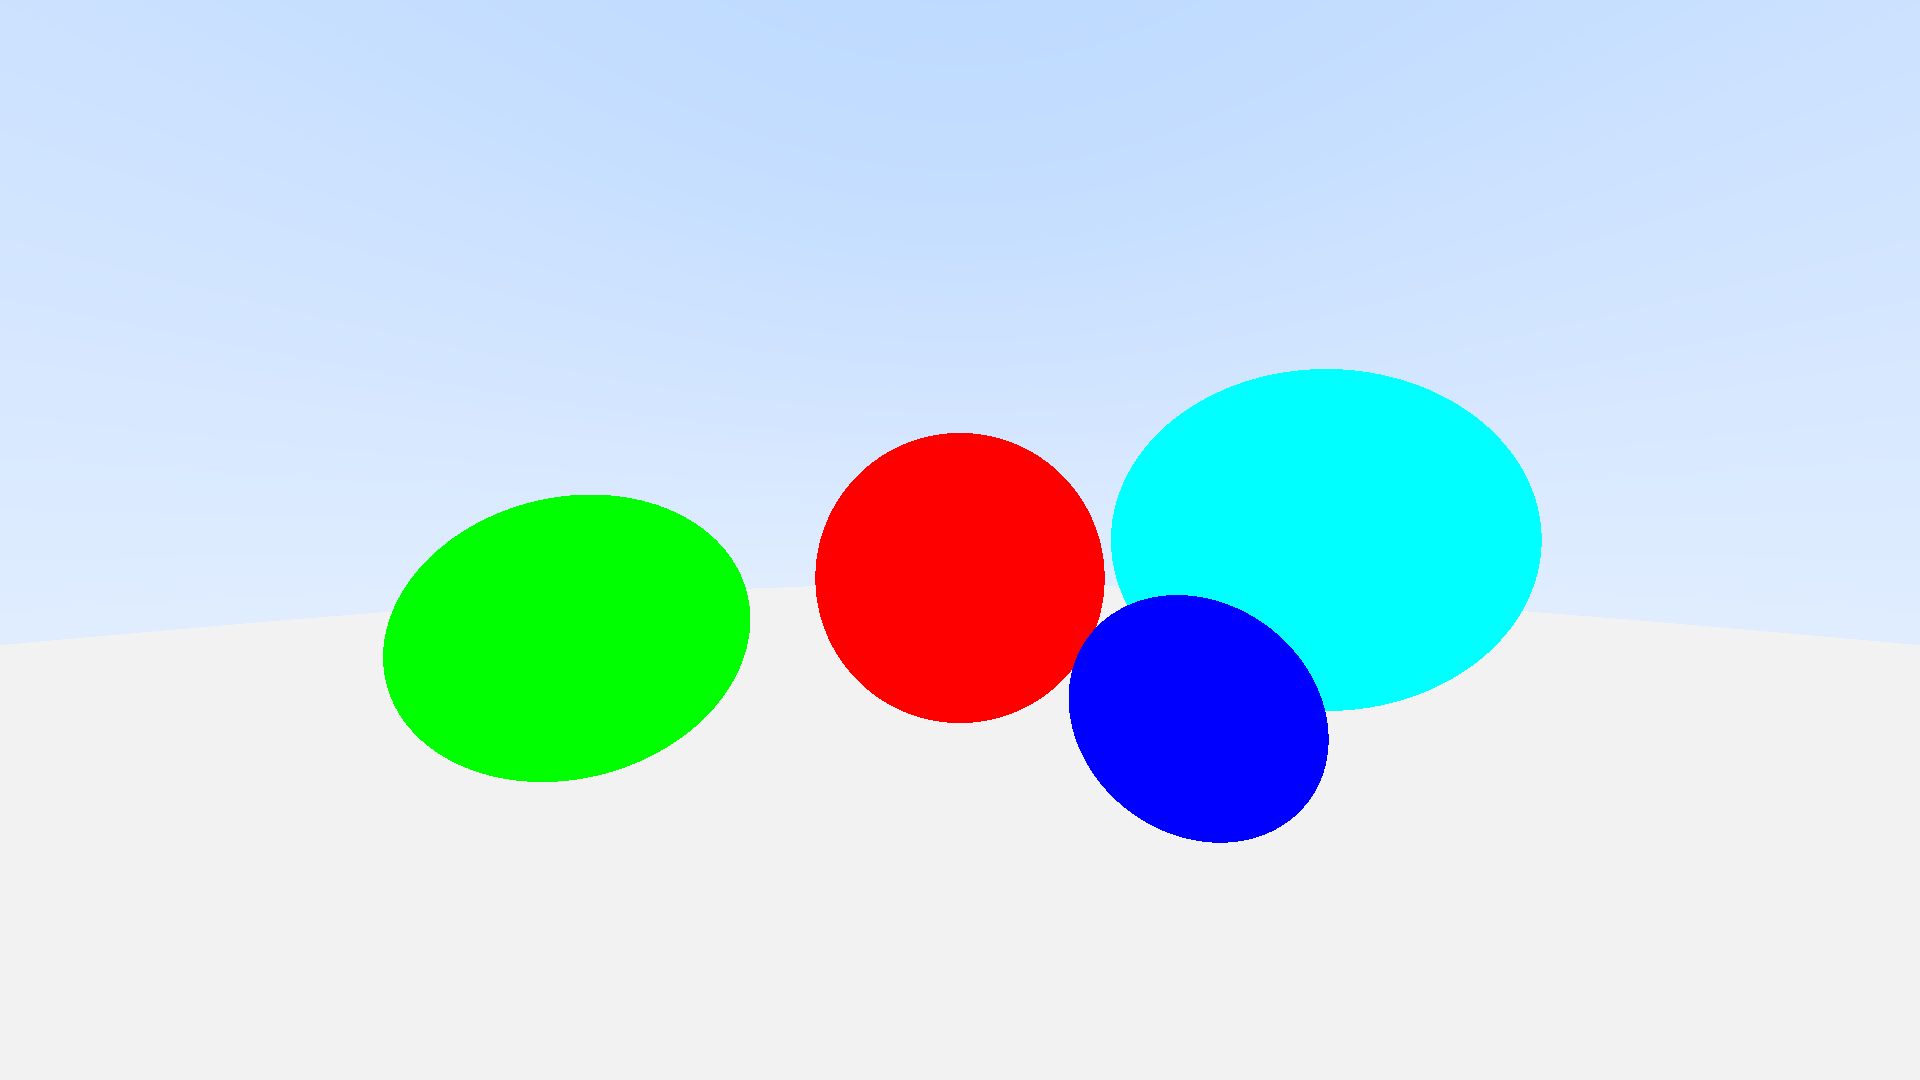
\includegraphics[width=0.75\linewidth]{image3}
		\caption{Scene of 5 spheres with different plain colors}
		\label{fig:image3}
	\end{figure}

	\subsection{Scene}
	\label{sec:scene}
	A 3D scene can contain a bunch of different objects which are rendered from one or more cameras. The \emph{Scene} class represents such a scene and allows to handle one or more cameras of \emph{Camera} class which render objects of \emph{RenderObject} class within the scene by calling the \emph{Scene} objects \emph{render()} function which is successively calling the cameras \emph{render()} functions. 
	\\
	This class is the interface for the user to generate the desired scene and render it within just on python file like for \emph{scene3.py} in \cref{lst:scene_example}.
	\begin{lstlisting}[caption={Example for Scene class usage from scene3.py}, language=Python, label=lst:scene_example]
from geometries import Vector
from objects import Scene, Camera, Sphere

scene = Scene("../images/image3")
# camera
main_camera = Camera(16 / 9, 1920, 1)

# spheres
s0 = Sphere(Vector(0, -1, -13), 4, color=Vector(1, 0, 0))
s1 = Sphere(Vector(-8, -2, -10), 3, color=Vector(0, 1, 0))
s2 = Sphere(Vector(4, -3, -8), 2, color=Vector(0, 0, 1))
s3 = Sphere(Vector(10, 0, -14), 5, color=Vector(0, 1, 1))
s4 = Sphere(Vector(0, -1005, -2), 1000, color=Vector(.9, .9, .9))

scene.add_render_object(s0)
scene.add_render_object(s1)
scene.add_render_object(s2)
scene.add_render_object(s3)
scene.add_render_object(s4)

scene.add_cam(main_camera)
scene.render()
	\end{lstlisting}
	
	\section{Antialiasing}
	\section{Materials}
		\subsection{Diffuse}
		\subsection{Specular}
		\subsection{Specular transmission}
		\subsection{Emissive}
	\section{Enhancing camera}
		\subsection{Positioning and orienting}
		\subsection{Depth of field}
	\section{Conclusion}
	
	\clearpage
	\addcontentsline{toc}{section}{References}
	\bibliography{./literature.bib}{}
	\bibliographystyle{plain}
		
\end{document}
